\chapter{Przegląd wybranych metod detekcji i~identyfikacji
obiektów w~obrazach}

We wstępie zamieszczono krótki opis pojęć detekcji i~identyfikacji.
Jednak ze względu na niejednoznaczności związane z~tymi terminami
zaobserwowane w~literaturze,
artykułach oraz dyskusjach na forach internetowych podjęto próbę
precyzyjnego określenia czym są: detekcja oraz identyfikacja
obiektów w~obrazach. Na potrzeby niniejszej pracy dyplomowej wprowadzone
zostały następujące dwie definicje.

Detekcja obiektów, innymi słowy wykrywanie lub lokalizacja,
polega na określeniu czy i~gdzie obiekt danej klasy występuje w~obrazie.
Jeżeli na obrazie widoczne są szukane obiekty,
produktem procesu powinny być współrzędne wszystkich ich wystąpień.
Przykładami tego typu działań są:

\begin{itemize}
    \item wykrywanie twarzy,
    \item detekcja przechodniów,
    \item lokalizacja tekstu w~scenie itp.
\end{itemize}

Identyfikacja (rozpoznawanie) obiektów polega na przypisaniu
poszczególnym instancjom już wykrytych obiektów odpowiadających im
etykiet. Dostarczone próbki w~założeniu powinny reprezentować
obiekty badanej klasy, czyli analogicznie do zaprezentowanych
przykładów z~dziedziny detekcji były by to: twarze,
znaki drukowane lub (niewymienione wcześniej) odciski palców.
Wynikiem tak zdefiniowanego działania powinny być nazwiska osób
skojarzonych z~twarzami lub odciskami palców,
czy w~przypadku znaków drukowanych odpowiadające im litery, cyfry
itp.

Idealnym podziałem z~punktu widzenia niniejszej pracy byłoby ścisłe
rozdzielenie algorytmów na dwie kategorie:

\begin{enumerate}
    \item Algorytmy odpowiadające na pytanie czy i~ewentualnie gdzie
        w~obrazie
        znajdują się obiekty szukanej klasy (z~uwzględnieniem przesunięcia,
        skalowania i~obrotu), na przykład twarze, znaki drogowe, znaki
        drukowane, samochody, fronty samochodów czy fronty autobusów.
    \item Algorytmy zwracające nazwę, typ lub identyfikator obiektu
        dostarczonego w~postaci określonej wielkości fragmentu obrazu
        w~ustalonej orientacji, na przykład przypisanie twarzy do
        właścicieli, znaku do kodu czy samochodu do marki i~modelu.
\end{enumerate}

Istnieje wiele algorytmów i~implementacji ściśle pasujących do
przedstawionych opisów. Są też jednak takie, które zawierają obie
funkcjonalności, na przykład śledzenie (detekcja) twarzy należącej
do konkretnej (identyfikacja) osoby. Niektóre rozwiązania zaprojektowane
w~celu detekcji po trywialnych modyfikacjach mogą służyć
do rozpoznawania wykrytych obiektów. Ostatecznie niektóre detektory
w~efekcie ubocznym mogą z~powodzeniem identyfikować poszczególne
instancje wykrywanych obiektów.

W~kolejnych podrozdziałach
przedstawiono najpopularniejsze algorytmy, implementacje
oraz koncepcje z~dziedziny detekcji i~identyfikacji obiektów w~obrazach.
Znaczna większość opisanych rozwiązań posiada gotową implementację
w~darmowej bibliotece OpenCV \cite{wiki:opencv}, która powstała
w~ramach projektu
zapoczątkowanego
w~1999 roku przez firmę Intel. W~2012 roku prace wznowiono
a~utrzymanie oraz rozwój powierzono fundacji non-profit
OpenCV.org. Biblioteka udostępniana jest wersjij
stabilnej 2.4.10 z~października 2014 oraz rozwojowej
3.0 BETA planowanej na maj 2014 (7 miesięcy opóźnienia).

Ze względu na licencję BSD, świetną
dokumentację, ciągły aktywny rozwój, implementację na wielu platformach,
w~tym Windwos, Linux oraz Android, jest to pozycja niezastąpiona
przy implementacji rozwiązań nie tylko z~dziedziny identyfikacji
i~detekcji lecz widzenia komputerowego w~ogóle. Dodatkowo nacisk
położony na przetwarzanie obrazów w~czasie rzeczywistym czyni z~biblioteki
OpenCV idealnego kandydata do wykorzystania w~implementacji
programu odczytującego numeru linii z~frontu nadjeżdżającego
autobusu na urządzeniu mobilnym z~systemem Android.

\section{Wykrywanie obiektów - detekcja}

Na potrzeby pracy wprowadzony i~opisany został termin
,,detekcji obiektów''. Na wejściu tak zdefiniowanego detektora
jest obraz zawierający (lub nie) wystąpienia interesujących obiektów, gdzie
wyjściem jest lista przyciętych obrazów reprezentujących wystąpienia tych
obiektów (fizyczne kopie lub współrzędne). W~kolejnych podrozdziałach
przedstawione zostały rozwiązania nawiązujące do powyższego opisu.

\subsection{Klasyfikator kaskadowy oparty na cechach Haara}

Struktura ramowa do wykrywania obiektów zaproponowana w~2001 roku, której
autorami byli Paul Viola i Michael Jones była pierwszą tego
rodzaju implementacją umożliwiającą wykrywanie obiektów w~czasie
rzeczywistym przy jednoczesnym zachowaniu wysokiej skuteczności
oferowanego rozwiązania. Algorytm został zaprojektowany z~myślą o~wykrywaniu
twarzy w~obrazie, nie uwzględnione było natomiast ich rozpoznawanie.
Główne jego zalety to m.in.:

\begin{itemize}
\item wysoka skuteczność - duży odsetek pozytywnych trafień brzy niewielkiej
ilości błędów,
\item wysoka wydajność - jak wspomniano we wstępie osiągnięto wyniki
rzędu kilkunastu klatek na sekundę dla obrazów wielkości 0.1Mpix na sprzęcie
klasy Pentium III,
\item możliwość przygotowania detektora dla innych obiektów, nie tylko
twarzy.
\end{itemize}

Co prawda rozwiązanie przewiduje proces przygotowywania detektorów
do wykrywania zadanych obiektów jednak trwa on długo - do kilku godzin lub dni
w~zależności od liczby próbek i~zadanych parametrów wejściowych. Dodatkowo
wymaga bardzo dużej liczby oznaczonych wystąpień interesujących obiektów
w~obrazach.
Autorzy pierwotnego rozwiązania wykorzystali zbiór kilku tysięcy
twarzy. Istnieją też opracowania w~których jest mowa o~kilkunastu lub nawet
kilkudzeisięciu tysiącach próbek pozytywnych.

Biblioteka OpenCV zawiera funkcje
do wykrywania obiektów w~językach Java, Python i~C++, oraz zestaw
programów pomocniczych
do przygotowywania
kaskadowych detektorów różnych typów. W~dokumentacji
\cite{OCV:cascadeclassification}
jest mowa o~dwuch opracowaniach \cite{DBLP:conf/cvpr/ViolaJ01,
DBLP:conf/icip/LienhartM02} na których bazuje oferowana
implementacja. Dostarczone narzędzia umożliwiają przogotowanie
detektorów opartych na cechach Haara, HOG oraz LBP (\textit{ang. Local Binary
Pattern}). Zastosowanie ostatniego z~wymienionych zestawu cech umożliwia
znaczne skrócenie czasu potrzebnego do przygotowania detektora.
Co ważne z~punktu widzenia tejże pracy, tak przygotowany detektor
charakteryzuje się też większą wydajnością, kosztem niewielkiego tylko spadku
dokładności, co przy wykorzystaniu odpowiednio dużej liczby próbek
podczas jego uczenia nie powinno mieć znaczenia.

Podstawowa funkcjonalność dostarczana przez implementację została zawarta
w~funkcji \verb|detectMultiScale|\cite{OCV:cascadeclassification}.
Dla przekazanego obrazu (argument wywołania)
zwracana jest kolekcja czworokątów okalających
reprezentująca wystąpienia szukanego obiektu.

Aby jednak skorzystać
ze~wspomnianej funkcji trzeba przygotować plik
definiujący klasyfikator. Jest to proces żmudny o~tyle, iż wymaga
dużej liczby oznaczonych wystąpień szukanych obiektów. Należy dostarczyć
tym dłuższą listę im większe zróżnicowanie w~obiektach reprezentujących
daną klasę. Jak już wspomniano liczba oznaczonych próbek powinna wynosić
co najmniej kilka tysięcy w~przypadku twarzy lub obiektów o~porównywalnej
rożnorodności. Przy czym zbiór obrazów tła (obrazy nie zawierające wystąpienia
szukanych obiektów)
powinien być równy co do ilości liczbie oznaczonych obiektów
lecz nie mniejszy niż ich połowa.

Kolejnym czynnikiem jest czas potrzebny na przygotowanie detektora.
Pierwotna metoda oparta na cechach Haara
jest najbardziej intensywna obliczeniowo, a~cały proces uczenia
może trwać do kilku dni. Rozwiązania oparte na innych cechach - LBP
(\textit{ang. Local Binary Pattern}) - ze względu na wykorzystanie
liczb całkowitych zamiast zmiennoprzecinowych trwają stosunkowo krócej, lecz
nadal czas wykonania liczony jest w~godzinach.

Samo wyszukiwanie obiektów oparte jest na oknie przesuwnym
(\textit{ang. sliding window}). Wspomniane okno przemieszcza się nad
obrazem definiując kombinację podobrazów, dla których po kolei uruchamiany
jest algorytm określający czy dany fragment reprezentuje szukany obiekt czy
nie. Ograniczeniem wprowadzonym przez to podejście jest brak możliwości
wykrycia obrotu, gdyż krawędzie okna są zawsze równoległe z~krawędziami
obrazu. Zaletą jest niewielka złożoność obliczeniowa, która pozwala
na wykrywanie i~lokalizowanie obiektów w~czasie rzeczywistym.

\subsection{Cechy 2D - struktura ramowa biblioteki OpenCV}

Biblioteka OpenCV poza wspomnianym detektorem udostępnia
strukturę ramową do operacji na cechach: ich wyliczanie, opisywanie
i~dopasowywanie \cite{OCV:feture2dframework}.
Tutaj w~odróżnieniu od detektora kaskadowego, zestaw cech
jest wyliczany dla każdego obrazu osobno i~jest to proces dużo bardziej
intensywny obliczeniowo niż w~poprzednim przypadku. Dodatkowo
funkcjonalność detekcji obiektów jest raczej efektem ubocznym,
a~ze względu na jednostkowy charaktery wyszukiwanych obiektów rozwiązanie
bardziej nadaje się do weryfikacji i~rozpoznawania obiektów niż do
detekcji i~lokalizacji obiektów pewnej klasy. Przykład zastosowania
zaprezentowano poniżej - rysunek \ref{fig:rev_features2d_detection}.

\begin{figure}[h!]
  \centering
    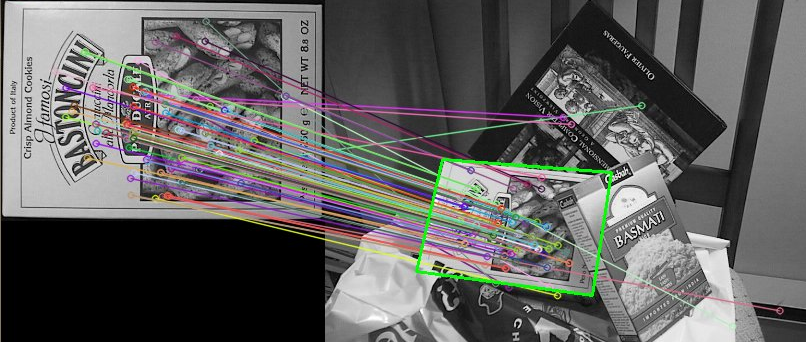
\includegraphics[width=0.8\textwidth]{img/rev_features2d_detection}
  \caption{Wykorzystanie framework-a cech 2d do wykrywania obiektów}
  \label{fig:rev_features2d_detection}
\end{figure}

Powyższy przykład pokazuje jak trudno zachować podział na wykrywanie
i~rozpoznawanie. Rysunek \ref{fig:rev_features2d_detection}
przedstawia przykład, gdzie wykrycie obiektu jest równoznaczne
z~jego rozpoznaniem.
Algorytm wylicza bowiem zestaw cech dla konkretnej okładki, po czym dla każdego
obrazu (w~przypadku pracy w~czasie rzeczywistym) wyliczany
jest dużo większy zestaw cech klatki. Jeżeli znaleziony zostanie
odpowiednio duży podzbiór cech podobnych na obu obrazach to wiadomo,
że obiek znajduje się w~kadrze.
Dodatkowo, na podstawie ułożenia pasujących cech, możliwe jest
wyznaczenie jego zniekształcenia geometrycznego. W~kontekście wprowadzonego
podziału jest to raczej przykład lokalizacji poszczególnych instancji danej
klasy obiektów niż wykrywanie obiektów klasy w~ogóle.
Poważnym
ograniczeniem jest wymóg posiadania dużej ilości szczegółów przez poszukiwany
obiekt, a~także wysoka rozdzielczość klatek w~obrębie których odbywa się
poszukiwanie. Złożoność obliczeniowa, a~co zatym idzie, czas przeszukiwania
poszczególnych klatek sprawiają, że metoda ta jest mało atrakcyjna w~kontekście
postawionego zadania.

Biblioteka OpenCV w~omawianym jej fragmencie posiada znacznie
większą niż wspomniana funkcjonalność.
Ze względu na mnogość zaimplementowanych algorytmów - których opis
wykracza poza zakres tego opracowania - istnieje ogromna ilość
zastosowań wspomnianego frameworka. Jednym z~nich jest na przykład
detekcja obszarów
reprezentujących tekst w~scenach naturalnych. W~tym celu
można wykorzystać implementację algorytmu MSER - (\textit{ang. Most
Stable Extreme Regions}) \cite{OCV:MSER}.

\subsection{Open TLD - detekcja i~identyfikacja}

Kelejnym algorytmem łączącym w~sobie funkcje wykrywania
i~rozpoznawania obiektów jest algorytm opracowany przez
Zdenka Kalala \cite{DBLP:journals/pami/KalalMM12} - TLD (\textit{ang.
Track Learn Detect}).

\begin{figure}[h!]
    \centering
    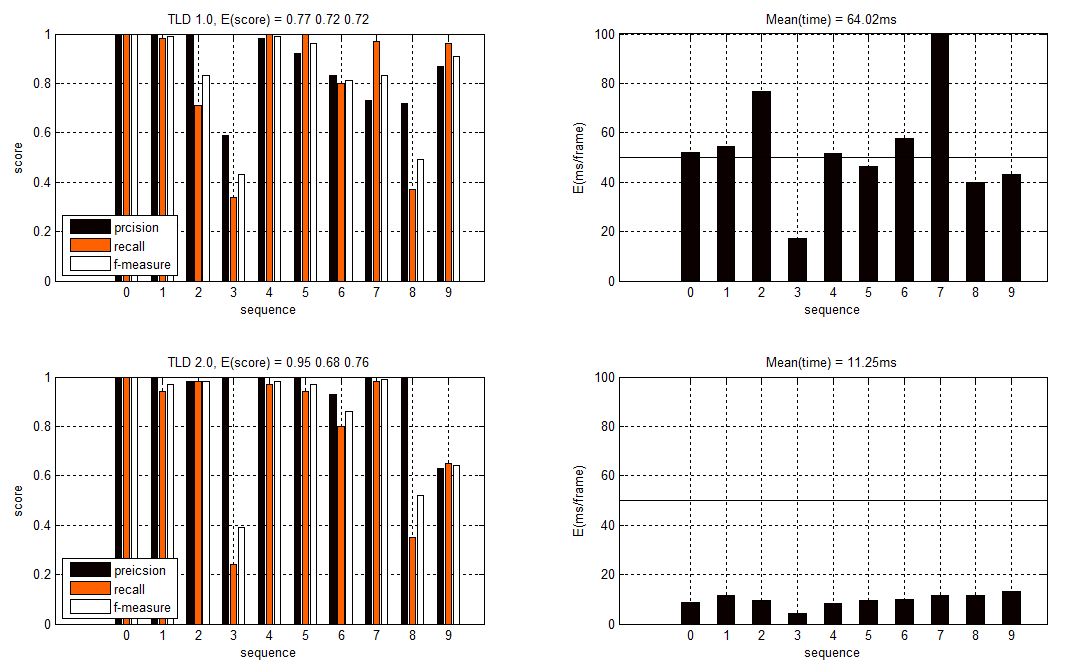
\includegraphics[width=1\textwidth]{img/rev_open_tld_1_2_comparison}
    \caption{Porównanie skuteczności i wydajności biblioteki OpenTLD w wersjach 1 i 2}
\end{figure}

Głównym zadaniem jakie rozwiązuje omawiany algorytm jest śledzenie obiektów.
Pewnym ograniczeniem jest potrzeba pierwszego oznaczenia interesującego
obiektu w~sekwencji obrazów tak aby możliwe było podjęcie pracy.
W~trakcie śledzenia tak oznaczonego obiektu odbywa się uczenie (doskonalenie)
detektora. O~ile sam etap śledzenia nie wykorzystuje detektora, to jest on
niezwykle istotny przy wznowieniu śledzenia po zniknięciu obiektu z~kadru.
Algorytm charakteryzuje się wysoką wydajnośćią i~zadziwiającą skutecznością.
Niestety wyniki naocznych eksperymentów i~zamieszczonych przez autorów filmów
demonstracyjnych wydają się być zbyt mało wiarygodne, szczególnie jeżeli
chodzi o~niezawodność.

Kolejną kwestią jest obecność gotowych implementacji.
Dostępna jest co prawda implementacja w~języku C/C++ oraz MatLabie. W~trakcie
pisania tego tekstu pojawiła się też druga wersja algorytmu niosąca
za sobą duże usprawnienia w~dziedzinie wydajności, co zaprezentowano
na wykresie poniżej.

Niestety brak implementacji w~pakiecie OpenCV lub
innej gotowej wersji dostępnej na system Android jest kolejnym
argumentem przeciwko wykorzystywaniu TLD jako elementu
programu odczytującego numer autobusu na urządzeniu z~systemem Android.
Wymagająca analiza i~naniesienie
niezbędnych modyfikacji
choć kształcące mogą nie przyczynić się do osiągnięcia zamierzonego celu.

Istnieje także przypuszczenie, że pozostawienie algorytmu w~trybie uczenia
może powodować powolny spadek wydajności ze względu na rosnącą liczbę
pozytywnych i~negatywnych obiektów w~bazie. Jest to jednak teza wymagająca
przeprowadzenia rzetelnych testów.

\section{Rozpoznawanie obiektów - identyfikacja}

Drugim terminem poza detekcją jest rozpoznawanie obiektów. Algorytm
identyfikacji najczęściej przyjmuje na wejściu obraz stałych rozmiarów
przedstawiający obiekt pewnej klasy. Zadaniem algorytmu jest zwrócenie
tekstu określającego typ, rodzaj lub po prostu nazwę danego obiektu.

Przykładem zastosowania może być odczytanie wykrytych liter,
cyfr, przypisanie twarzy do właścicieli lub zwrócenie marki wykrytego
samochodu.

Ze względu na specyfikę zagadnienia gotowych implementacji algorytmów
identyfikacji jest niewiele lub sprawdzają się one w~obrębie
ściśle określonego zagadnienia. Niektóre z~przytoczonych w~poprzednim
podrozdziale przykładów mogą równie dobrze służyć jako identyfikatory
obiektów. Algorytm OpenTLD skutecznie rozróżnia twarze, gesty oraz
poszczególne instancje obiektów różnych klas.

Klasycznym podejściem do identyfikacji jest uczenie maszynowe. Na
wejściu podawany jest zbiór reprezentantów poszczególnych klas
z~przypisanymi do nich oczekiwanymi rezultatami. Rozwiązanie
sprawdza się przy rozpoznawaniu znaków drukowanych o~wysokim
kontraście i~w~wysokiej rozdzielczości. Ograniczeniem jest bowiem
potrzeba wprowadzenia pojęcia odległości między poszczególnymi
reprezentantami danej klasy. Wykorzystując do tego bibliotekę
OpenCV \ można wybrać dwie metody:

\begin{itemize}
\item K-najbliższych-sąsiadów,
\item SVM.
\end{itemize}

Obie metody są podobne. Zakładają fazę uczenia i~rozpoznawania.
Jednak obliczanie odległości pomiędzy dwoma instancjami obiektu
i~wybór odpowiedniej metody ku temu pozostaje w~gestii programisty.
Niestety może to być dowolna metoda. Można użyć deskryptorów cech
SIFT, SURF, BRIEF itp. W~skrajnie laboratoryjnych warunkach, tak
jak w~odczytywaniu znaków czarno-białych można porównywać poszczególne
piksele i~obliczać w~prost różnicę między obrazami. Jeżeli jednak tekst
jest ulokowany w~tak zwanej scenie naturalnej -
szyld, reklama, bilbord itp. - różnice w~czcionkach, refleksy
i~zniekształcenia uniemożliwiają wykorzystanie tak trywialnej metody.
Zagadnienie jest na tyle ważne i~jednocześnie skomplikowane, że
powstał plebiscyt, którego zadaniem jest wyłonienie najlepszego
algorytmu odczytującego teksty ze scen naturalnych. Odbywa się
on co dwa lata, a~ostatnia edycja miała miejsce w~roku 2013.
Zwycięzcy konkursu ICDAR2013 w~dziedzinie odczytywania tekstu ze
zdjęć, do rozpoznawania poszczególnych znaków wykorzystali sieci neuronowe.
Podobnie było w~przypadku algorytmu odczytującego numery domów na potrzeby
geolokalizacji w~usłudze Google:StreetView. Ostatecznie zadanie
odczytywania numerów/tekstów ze zdjęć jest zadaniem najtrudniejszym
z~dotąd omawianych.

\begin{figure}[h!]
    \centering
    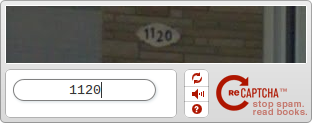
\includegraphics[width=0.8\textwidth]{img/rev_captcha_street_view}
    \caption{Przykładowa captcha z prawdopodobnym numerem domu}
\end{figure}

O~skali złożoności problemu może świadczyć fakt, iż
opracowany przez Google algorytm wymaga wspomagania w~postaci
ręcznej interwencji
operatorów. Przeglądając zasoby internetu napotkana została captcha
z~obrazkiem przypominającym numer domu, co może świadczyć, że stuprocentowa
automatyzacja rozpoznawania numerów domów nie do końca udała się inżynierom
z Mountain View.

